\documentclass[t,compress,aspectratio=169]{beamer}
\usetheme{neutral}

\usepackage[english]{babel}
\usepackage[utf8]{inputenc}
% \usepackage[lighttheme]{uobham-beamer}
\usepackage{listings}
\usepackage[UKenglish]{datetime}
\usepackage{algpseudocode}
\usepackage{fontawesome5}
\usepackage{listings}
\usepackage{multirow}
\usepackage{booktabs}
\usepackage{soul}
\usepackage{minted}
%\usepackage{local-macros}

\newcommand{\translation}{\mathbf{T}}


%Matthew's - need to go through and swap some stuff, rename some
% \newcommand{\Bool}{\mathbb{B}}
% \newcommand{\Nat}{\mathbb{N}}
% \newcommand{\id}{x}
% \newcommand{\val}{a}
% \newcommand{\cons}[2]{#1 :: #2}
% \newcommand{\consNew}[2]{#2[#1]}

\newcommand{\vehicle}[1]{{\mintinline{haskell}{#1}}}

\usepackage{ulem}
\newdateformat{UKvardate}{%
	\monthname[\THEMONTH] \THEDAY \ \THEYEAR}

% Set to 1 or comment to disable transparency and enable full opacity.
\setblockbodyopacity{0.8}

% Listings
\definecolor{cident}{rgb}{1,0.33,0.42}
\definecolor{ckeyw}{rgb}{1,0.2,0.8}
\definecolor{ccomm}{rgb}{0,0.8,0}
\definecolor{cstr}{rgb}{0.8,0,0}

\lstset{language=[LaTeX]{TeX},
  basicstyle=\footnotesize\ttfamily,
  keywordstyle=\color{ckeyw}\bfseries,
  identifierstyle=\color{cident}\bfseries,
  commentstyle=\color{ccomm},
  stringstyle=\color{cstr},
  showstringspaces=false,
  breaklines=true,
  breakatwhitespace=true,
  tabsize=2,
%   numbers=left,
%   stepnumber=1,
%   firstnumber=1,
%   numberfirstline=true,
  }

\usepackage{stmaryrd}
\usepackage{local-macros2}
\newcommand{\distance}[2]{|#1 - #2|}
\newcommand{\outputdistance}[2]{||#1 - #2||}
%\newcommand{\x}{\vect{x}} 		% Arbitrary input
%\newcommand{\xt}{\hat{\x}} 		% Training input
\newcommand{\xs}{\x} 			% Sampled input
\newcommand{\xp}{\tilde{\x}} 	% Perturbed input

%\newcommand{\y}{\vect{y}} 		% Arbitrary output
\newcommand{\yt}{\hat{\y}} 		% Training output
\newcommand{\ys}{\y} 			% Sampled output



\newcommand{\SR}[2]{SR(#1, #2)} % Standard robustness
\newcommand{\LR}[2]{LR(#1, #2)} % Lipschitz robustness
\newcommand{\CR}[1]{CR(#1)} % Classification robustness
\newcommand{\SCR}[2]{SCR(#1,#2)} % Approximate class. robustness
\usepackage{pifont}
\definecolor{forestgreen}{RGB}{35, 142, 35}
\definecolor{lightaisecred}{RGB}{237, 41, 57}
\newcommand{\yes}{\textcolor{forestgreen}{\ding{51}}}
\newcommand{\no}{\textcolor{aisecred}{\ding{55}}}
\newcommand{\good}[1]{\textcolor{forestgreen}{#1}}
\newcommand{\average}[1]{\textcolor{orange}{#1}}
\newcommand{\bad}[1]{\textcolor{aisecred}{#1}}

\newcommand{\wrapp}[2]{\begin{minipage}[t]{#1\columnwidth}
    \centering #2
\end{minipage}}


\usepackage{amsfonts,amsmath,amssymb,amsthm}
\usepackage[all]{xy}
\usepackage{array,url}
\usepackage{textcomp,textgreek}
\usepackage{pgfplots}
\usepackage{float}
\pgfplotsset{width=5cm,compat=1.9}
\usepackage{mdframed,wrapfig,subcaption}
%\usepackage[font=footnotesize,labelfont=it
%\usepackage[latin1]{inputenc}
\usepackage{babel}
\usepackage{color}
%\usepackage{url}
\usepackage{hyperref}
\usepackage{fancyvrb}
%\usepackage{tikz}
\usepackage{alltt}
%\usepackage{etex, xy}
%\usepackage{cibeamer}
\usepackage{tikz}
\usetikzlibrary{arrows,shapes}
%\xyoption{all}
%\usepackage{listings}
%\input macro
\usepackage{cancel, comment}
\usepackage{verbatim}
\usepackage{slashbox}
\usepackage{ulem}

\newcommand{\tikzmark}[1]{\tikz[remember picture] \node[coordinate] (#1) {#1};}
\newcommand{\semitransp}[2][35]{\color{fg!#1}#2}

\usepackage[absolute,overlay]{textpos}
\beamertemplatenavigationsymbolsempty
\usepackage{ijcnn-diagram}

\usepackage[all]{foreign}

\newcommand{\fstar}{F$^\ast$\xspace}
\newcommand{\starchild}{StarChild\xspace}
\newcommand{\lazuli}{Lazuli\xspace}
\newcommand{\sapphire}{Sapphire\xspace}
\newcommand{\cL}{{\cal L}}
%\newcommand{\Real}{{\mathbb R}}
\usepackage{makecell}
\DeclareMathOperator{\linear}{linear}
\DeclareMathOperator{\relu}{relu}
\DeclareMathOperator{\sigmoid}{sigmoid}
\DeclareMathOperator{\softmax}{softmax}
\DeclareMathOperator{\neuron}{neuron}
\DeclareMathOperator{\truthy}{truthy}
\DeclareMathOperator{\falsey}{falsey}
\DeclareMathOperator{\neurontest}{test}
\usepackage{ellipsis}
\renewcommand{\ellipsisgap}{-0.25em}



\colorlet{MyColour}{teal}

\newcommand{\coloured}[1]{\textcolor{MyColour}{#1}}


\definecolor{beamer@headercolor}{RGB}{204, 72, 71}
\colorlet{beamer@barcolor}{beamer@headercolor!70!black}

\definecolor{beamer@progresscolor}{HTML}{ffe960}
%\setbeamercolor{AAUsimple}{fg=aisecred!20,bg=aisecred}
%\setbeamercolor{sidebar}{bg=aisecred!20}
% Change the color of the structural elements:
%\setbeamercolor{structure}{fg=aisecred}
% Change the frame title text color:
\setbeamercolor{frametitle}{fg=aisecpurple!20!black}
\setbeamercolor{definition}{fg=aisecaisecred!10!white}


% Change the normal text color background:
\setbeamercolor{normal text}{fg=black,bg=gray!10}
\setbeamercolor{subtitle}{fg=white!90!aisecpurple,bg=gray!10}

\usepackage{soul}
\makeatletter
\let\HL\hl
\renewcommand\hl{%
  \let\set@color\beamerorig@set@color
  \let\reset@color\beamerorig@reset@color
  \HL}
\makeatother

%\usetikzlibrary{decorations.pathreplacing,shapes.arrows}
\newcommand\BackgroundPicture[1]{%
  \setbeamertemplate{background}{%
   \parbox[c][\paperheight]{\paperwidth}{%
      \vfill \hfill
\includegraphics[width=1\paperwidth,height=1\paperheight]{#1}
        \hfill \vfill
     }}}
\usepackage{xcolor,colortbl}
%\usepackage{listings}
\definecolor{Gray}{gray}{0.85}

\newcommand{\question}[1]{\begin{description}
		\item[\textbf{Question.}] #1
\end{description}}

\newcommand{\task}[1]{\begin{description}
		\item[{\textcolor{aisecred}{\textbf{Task.}}}] #1
\end{description}}

\newcommand{\focus}[1]{\begin{description}
		\item[{\textcolor{aisecred}{\textbf{Note.}}}] #1
\end{description}}


\def\checkmark{\tikz\fill[scale=0.4,color=green](0,.35) -- (.25,0) -- (1,.7) -- (.25,.15) -- cycle;}
\newcommand{\down}[1][aisecred]{{\color{#1}\scalebox{1.4}[.7]{\,$\blacktriangledown$\,}}}
\newcommand{\up}[1][green!70!black]{{\color{#1}\raisebox{0.1em}{\scalebox{1.4}[.7]{\,$\blacktriangle$\,}}}}
\newcommand{\stall}[1][yellow!70!aisecred]{{\color{#1}\raisebox{0.1em}{\scalebox{1.4}[.5]{\,$\blacksquare$\,}}}}

\title{Neural Network Verification With Vehicle: Chapter 4 -  Property-Driven Training}

\subtitle{ICFP'23 Tutorial}  % could also be a conference name

\date{\today}

\author{Matthew Daggitt  \inst{1} \and Wen Kokke (online) \inst{2}  \and Ekaterina Komendantskaya\inst{3}}

\institute{$^{1}$Heriot-Watt University $\cdot$ $^{2}$University of Strathclyde $\cdot$  $^{3}$University of Southampton }

\setbackgroundgraphics{img/Seattle}
\setbackgroundgraphicscopy{image by \copyright {\bf Visit the USA}}
% \setlogographics{img/artwork-logo}
% \settitlegraphics{img/cloud}

\setcirclelogographics{img/artwork-logo-circle}

% specify a logo on the titlepage (you can specify additional logos an include them in
% institute command below
% \pgfdeclareimage[height=2cm]{titlepagelogo}{\logographics} % placed at the title page
% % \pgfdeclareimage[height=7cm]{titlepagelogo2}{\titlegraphics} % placed on the title page


% \titlegraphic{% is placed at the bottom of the title page
%   \pgfuseimage{titlepagelogo}
% %   \pgfuseimage{titlepagelogo2}

% %  \hspace{1cm}\pgfuseimage{titlepagelogo2}
% }


\begin{document}
% the titlepage

\setbackground
\begin{frame}[fragile,plain,noframenumbering] % the plain option removes the header from the title page
  \titlepage
\end{frame}
\unsetbackground


\begin{frame}
\frametitle{In this chapter...}

We will discuss:

\begin{itemize}[<+->]
\item  ...  why and how training is a part of verification of neural networks
\item ... what choices exist for implementing this, generally
\item ... what choices \textbf{Vehicle} makes in this respect
\item ... theoretical and practical issues with the chosen methods, and \textbf{Vehicle}'s
take on them
\end{itemize}

\end{frame}


\begin{frame}
\frametitle{Recap: four PL problems}

\begin{itemize}
\item[$I^O$] \alert{Interoperability -- properties are not portable between training/counter-example search/ verification.}

\item[$I^{P}$] Interpretability -- code is not easy to understand.

\item[$I^{\int}$] Integration -- properties of networks cannot be linked to larger control system properties.

\item[$E^G$] Embedding gap -- little support for translation between problem space and input space.
\end{itemize}
\end{frame}


    \begin{frame}[fragile]
\frametitle{Why Training is a part of Verification?}

\begin{minted}[fontsize=\footnotesize]{haskell}
vehicle verify \
  --specification acasXu.vcl \
  --verifier Marabou \
  --network acasXu:acasXu_1_7.onnx \
  --property property3

Verifying properties:
property3 [==========================================] 1/1 queries
  result:  counterexample found
  x: [1799.9886669999978, 1.9509286320000003e-2,
                        3.09999732192, 980.0, 1017.6036]
\end{minted}

\end{frame}

   \begin{frame}
\frametitle{Why Training is a part of Verification?}

Verifying a Fashion MNIST network on $500$ samples we get:

 ~

\hrule

~

\footnotesize{
\begin{tabular}{|p{0.15\textwidth}|p{0.2\textwidth}|p{0.2\textwidth}|p{0.15\textwidth}| p{0.15\textwidth}|}
		\hline
& 	$\epsilon = 0.01$ & $\epsilon = 0.05$ & $\epsilon = 0.1$ & $\epsilon = 0.5$ \\ \hline \hline

Success rate: & 82.6 \% (413/500) &	29.8 \% (149/500) &	3.8 \% (19/500) & 	0 \% (0/500)\\
		 \hline
	\end{tabular}}


\end{frame}

\begin{frame}
  \frametitle{A few words on the context}
\vspace{-2em}
  \begin{itemize}
  \item[1943] Perceptron by McCullogh and Pitts
  \item[90-2000] Rise of machine learning applications
  \item[2013]
   {\scriptsize
 \begin{thebibliography}{99}
 \beamertemplatearticlebibitems
  \bibitem{2}{C.~Szegedy, W.~Zaremba, I.~Sutskever, J.~Bruna, D.~Erhan,
I.~Goodfellow, and R.~Fergus.  Intriguing properties of neural networks. 2013. (10000+ citations on GS)}
\end{thebibliography}}

\item[2013-..] Tens of thousands of papers on adversarial training

  (in the attack-defence style)
    {\scriptsize
 \begin{thebibliography}{99}
   \beamertemplatearticlebibitems
   \bibitem{3}{A.~C.~Serban, E.~Poll, J.~Visser.
Adversarial Examples - A Complete Characterisation of the Phenomenon. 2019.}
\end{thebibliography}}

\pause

\item[2017] First Neural network verification attempts
    {\scriptsize
 \begin{thebibliography}{99}
   \beamertemplatearticlebibitems
    \bibitem{4}{G.~Katz, C.W.~Barrett, D.L.~Dill, K.~Julian, M.J.~Kochenderfer:
      Reluplex: An Efficient SMT Solver for Verifying Deep Neural Networks. CAV (1) 2017: 97-117.}
    \bibitem{5}{ X. Huang, M. Kwiatkowska, S. Wang, M. Wu. Safety Verification of Deep Neural Networks. CAV (1) 2017: 3-29.}
\end{thebibliography}}


\item[2017-..] Hundreds of papers on neural network verification

  \end{itemize}
\end{frame}




\begin{frame}
  \frametitle{Training for Robustness}
    Training generally:

    \begin{enumerate}
    \item depends on data
    \item depends on loss functions
      \item some other parameters like shape of the functions
      \end{enumerate}

\end{frame}





\begin{frame}[fragile]
  \frametitle{1. Data Augmentation}
  \vspace{-1em}
  Suppose we are given a data set $\mathcal{D} =  \{(\x_1, \y_1), \ldots , (\x_n, \y_n)\}$. \\
  Prior to training, generate new training data samples close to existing data\\ and label them with the same output as the original data.
      {\scriptsize
 \begin{thebibliography}{99}
   \beamertemplatearticlebibitems
    \bibitem{6}{C. Shorten, T.M. Khoshgoftaar:
       A survey on image data augmentation for deep learning. J.
Big Data 6, 60 (2019)}
\end{thebibliography}}

\pause

\begin{center}

  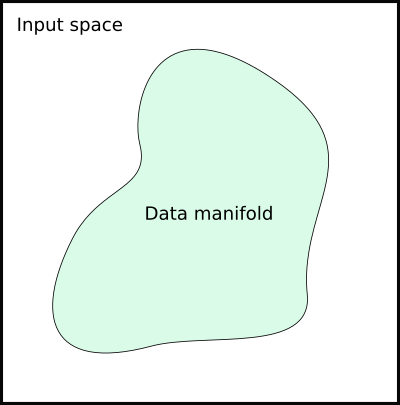
\includegraphics[width=4cm]{img/SR-vs-CR-1.png}

  \end{center}

\end{frame}


\begin{frame}[fragile]
  \frametitle{1. Data Augmentation}

    \vspace{-1em}



  Suppose we are given a data set $\mathcal{D} =  \{(\x_1, \y_1), \ldots , (\x_n, \y_n)\}$.
  Prior to training, generate new training data samples close to existing data and label them with the same output as the original data.
      {\scriptsize
 \begin{thebibliography}{99}
   \beamertemplatearticlebibitems
    \bibitem{6}{C. Shorten, T.M. Khoshgoftaar:
       A survey on image data augmentation for deep learning. J.
Big Data 6, 60 (2019)}
\end{thebibliography}}


\begin{center}

  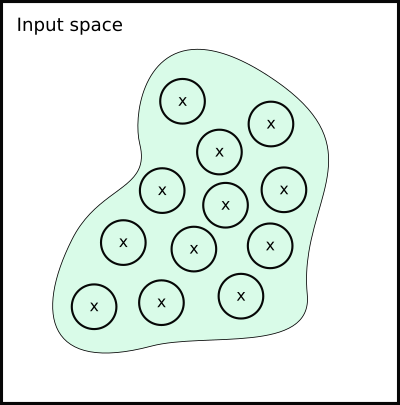
\includegraphics[width=4cm]{img/SR-vs-CR-2.png}

  \end{center}

\end{frame}




\begin{frame}[fragile]
  \frametitle{However,}
  \vspace{-1em}


\begin{center}

  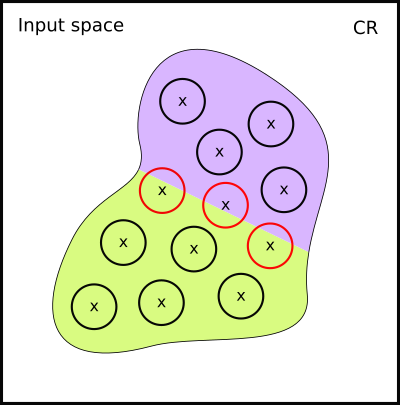
\includegraphics[width=4cm]{img/SR-vs-CR-4.png}

  \end{center}

\end{frame}


\begin{frame}[fragile]
  \frametitle{However,}

  \vspace{-1em}


\begin{center}

  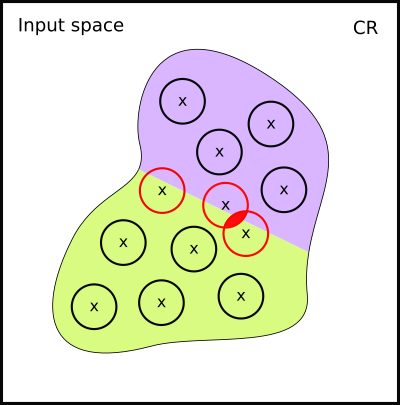
\includegraphics[width=4cm]{img/SR-vs-CR-5.png}

  \end{center}

 \end{frame}

 \begin{frame}[fragile]
  \frametitle{Adversarial Training}


  \vspace{-1em}

\begin{center}

  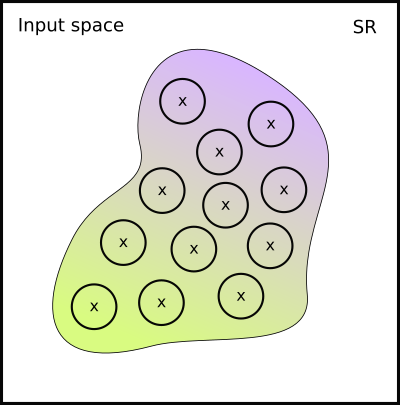
\includegraphics[width=4cm]{img/SR-vs-CR-3.png}

  \end{center}
   {\scriptsize
   \begin{thebibliography}{99}
        \beamertemplatearticlebibitems
    \bibitem{7}
I.J. Goodfellow, J. Shlens, C. Szegedy: Explaining and harnessing adversarial examples. 3rd International Conference on Learning Representations,
ICLR 2015, San Diego, CA, USA, May 7-9, 2015, Conference Track Proceedings (2015)
 \end{thebibliography}}
 \end{frame}


\begin{frame}
  \frametitle{2. Solutions Involving Loss Functions}
    \vspace{-2em}

Given a data set $\mathcal{D} $,\\  a function  ${f_{\theta}: \Real^n \rightarrow \Real^m}$ (with optimisation parameters $\theta$),\\
	a \emph{loss function} $\losssymbol: \Real^n \times \Real^m \rightarrow \mathbb{R}$ computes a penalty proportional to the difference between the output of $f_{\theta}$ on a training input $\xt$ and a desired output $\y$.\pause


\begin{example}[Cross Entropy Loss Function]
	\label{eq:cross-entropy}
	Given a function  ${f_{\theta}: \Real^n \rightarrow [0,1]^m}$, the cross-entropy loss is defined as
	\begin{equation}\label{eq:ce}
	\losssymbol_{ce}(\xt, \y) = - \sum_{i=1}^{m} \y_i \; \log(f_{\theta}(\xt)_i)
	\end{equation}
	where $\y_i$ is the true probability for class $i$ and $f_{\theta}(\xt)_i$ is the probability for class $i$ as predicted by $f_{\theta}$ when applied to $\xt$.
\end{example}

\end{frame}



\begin{frame}
  \frametitle{2. Adversarial Training  for Robustness}

\vspace{-2em}
  \begin{itemize}
  \item  \emph{gradient descent}  minimises loss $\lossfn(\xt, \y)$ between\\ the predicted value $f_{\theta}(\xt)$ and the true value $\y$, for each entry $(\xt, \y)$ in $\mathcal{D}$.\\ It thus solves the optimisation problem:
  $$ \min_{\theta} \lossfn(\xt, \y) $$
  \pause
  \item For \emph{adversarial training}, we instead minimise the loss with respect to the worst-case perturbation of each sample in $\mathcal{D}$.
\begin{itemize}
     \item Replace the standard training objective with:
%\begin{equation}
$$\min_{\theta} [ \max_{\xs : \distance{\xs}{\xt} \leq \epsilon} \lossfn(\xs, \y)]$$
 \item the inner maximisation is done by \emph{``projected gradient descent"} (PGD), that ``projects" the gradient of $\mathcal{L}$ on $\xt$ in order to perturb it and get the worst $\xs$.

\end{itemize}
\end{itemize}

 {\scriptsize
   \begin{thebibliography}{99}
        \beamertemplatearticlebibitems
    \bibitem{7}
    Zico Kolter and Aleksander Madry. Adversarial Robustness - Theory and Practice. NeurIPS 2018 tutorial.

 \end{thebibliography}}

\end{frame}


    \begin{frame}
      \frametitle{ Lipshitz Continuity}

      Optimise for:

  \begin{equation*}
    \label{eq:lipschitz-robustness}
    \forall \xs: \distance{\xs}{\xt} \leq \epsilon \Rightarrow \distance{f(\xs)}{f(\xt)} \leq L \distance{\xs}{\xt}
  \end{equation*}

   {\scriptsize
   \begin{thebibliography}{99}
        \beamertemplatearticlebibitems
    \bibitem{7}
P. Pauli, A. Koch, J. Berberich, P. Kohler, F. Allgower: Training robust neural networks
using Lipschitz bounds. IEEE Control Systems Letters (2021)
\bibitem{8} H. Gouk, E. Frank, B. Pfahringer, M.J. Cree: Regularisation of neural networks by enforcing Lipschitz continuity. Machine Learning 110(2), 393–416 (2021)
\end{thebibliography}}


and much more...

    \end{frame}


 \begin{frame}
      \frametitle{3. Other ways to do property-driven training}

\begin{block}{More sophisticated approaches to property driven training include:}
\begin{itemize}
\item Tailoring the neural network architectures

\item Tailoring the activation functions

\item Including probabilsitic or deterministic solvers into neural network layers

\item $\ldots$
\end{itemize}
\end{block}

  {\scriptsize
 \begin{thebibliography}{99}
   \beamertemplatearticlebibitems
    \bibitem{6}{Eleonora Giunchiglia, Mihaela Catalina Stoian, and Thomas Lukasiewicz. Deep learning
with logical constraints. IJCAI 2022, pages 5478–5485. ijcai.org, 2022}
\end{thebibliography}}



\end{frame}

\begin{frame}
\frametitle{}
\vspace{5em}
\begin{alertblock}{Ok, great!}
 Machine Learning Community knows how to make our networks more robust, and maybe even verifiable!
\end{alertblock}
\pause
But remember:

\begin{block}{}
\begin{itemize}
\item[$I^O$] \alert{Interoperability -- properties are not portable between training/counter-example search/ verification.}

\item[$I^{P}$] \alert{Interpretability} $\ldots$

\item[$I^{\int}$] Integration $\ldots$

\item[$E^G$] Embedding gap $\ldots$
\end{itemize}
\end{block}
\end{frame}

\begin{frame}
  \frametitle{Interpretation of adversarial training:}
  \vspace{-2em}
   % \begin{itemize}[<+-|alert@+>]
      \begin{block}{Recall the epsilon ball robustness:}

       $\forall \x \in \mathbb{B}(\hat{\x}, \epsilon). \ \alert{robust}(f(\x)) $
\end{block}

     We can map different kinds of adversarial training to formal properties:
\begin{tabular}{p{3.5cm}|p{4cm}| p{4cm}}
%\toprule
Training style & Definition of \alert{$robust$} & Property \\ \hline \hline
%\midrule
Data Augmentation & 	$ argmax\ [f(\x)] = i$  & Classification Robustness\\ \hline
DL2 training & 	$f(\x)_i \geq \eta$  & Strong Classification Robustness \\ \hline
Adversarial Training & 	$ |f(\x) - f(\hat{\x})| \leq \delta$ & Standard Robustness\\ \hline
Lipschitz Continuity & 	$ |f(\x) - f(\hat{\x})| \leq L|\x-\hat{\x}|$ & Lipschitz Robustness \\ \hline
          ... & ... &  ... \\

		%\bottomrule
	\end{tabular}
    %    \end{itemize}


       {\scriptsize
 \begin{thebibliography}{99}
   \beamertemplatearticlebibitems
    \bibitem{6}{M. Casadio, E. Komendantskaya, M. L. Daggitt, W. Kokke,
G. Katz, G.~Amir, and I.~Rafaeli. 2022. Neural Network Robustness as a Verification Property:
A Principled Case Study. CAV'22.}
\end{thebibliography}}




  \end{frame}




\begin{frame}[fragile]
\frametitle{Consequences of this finding:}

\begin{itemize}[<+->]
\item one kind of robustness does not necessarily imply another;

\item It is easy to get it wrong, and,  while optimising for \alert{one kind} of robustness, achieve little in verification success rates

\begin{example}
In majority of ML + verification papers, adversarial robustness is used for training (it encourages \emph{standard robustness of networks}), while verification is done for \emph{classification robustness}. We show that these two types of robustness are not in any relation: i.e. increasing one does not generally increase the other.
\end{example}

\item And what to do with properties that are not $\epsilon$-ball robustness? Out-of-the-box PGD training only works with $\epsilon$-balls around data points.
\end{itemize}



\end{frame}

\begin{frame}
	\frametitle{The solution we are looking for}
	\vspace{-2em}
	\begin{figure}[t]
		\begin{center}
			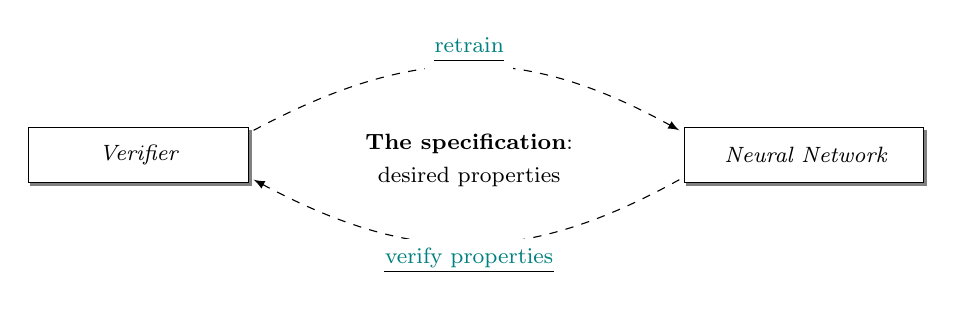
\begin{tikzpicture}[scale=.7]

				\draw[fill=gray,draw=gray] (-2.95,.45) rectangle (1.05,-.55);
				\draw[fill=white] (-3,.5) rectangle (1,-.5);
				\node (0,0) { };
				\draw (-1,0) node {{\footnotesize \it Verifier} };

				\draw[fill=gray,draw=gray] (8.95,.45) rectangle (13.30,-.55);
				\draw[fill=white] (8.9,.5) rectangle (13.25,-.5);
				\draw (11.1,0) node{{\footnotesize \it Neural Network}};


				\draw (5,0.2) node{\footnotesize{\textbf{The specification}:}};
				\draw (5,-0.4) node{\footnotesize{desired properties}};


				\draw[latex-,shorten <=2pt,shorten >=2pt,dashed] (8.9,.4) .. controls (6,2) and (4,2) .. (1,.4);
				\draw (5,2.3) node[anchor=north,fill=white]{\emph{\footnotesize{\textcolor{teal}{retrain}}}};

				\draw[latex-,shorten <=2pt,shorten >=2pt,dashed] (1,-.4) .. controls (4,-2) and (6,-2) .. (8.9,-.4);
				\draw (5,-2.3) node[anchor=south,fill=white]{\emph{\footnotesize{\textcolor{teal}{verify properties}}}};
			\end{tikzpicture}
		\end{center}
	\end{figure}
	\pause
	\begin{block}{NB}
\begin{itemize}
\item[$I^O$] \alert{Interoperability} $\ldots$

\item[$I^{P}$] \alert{Interpretability} $\ldots$

\item[$I^{\int}$] Integration $\ldots$

\item[$E^G$] Embedding gap $\ldots$
\end{itemize}
\end{block}

\end{frame}

\begin{frame}
\frametitle{In Vehicle terms,}

\vspace{-2em}
\begin{center}
\begin{tikzpicture}[thick,
    set/.style = {circle,
        minimum size = 3cm}]

% Set A
\node[rectangle,draw] (A) at (1.5,5) {\alert{Property in Vehicle}};

\node[rectangle,draw] (B) at (-3,2) {\alert{Training}};
\node[text width=2cm, align=center] at (-3,0) {\alert{DL2 or other DL (native)}};

\node[rectangle,draw, dashed,text width=1.4cm] (C) at (0,2) {\alert{Counter-example search}};
\node[text width=1cm, align=center] at (0,0) {\alert{PGD FGSM etc.}};

\node[rectangle,draw] (D) at (3,2) {Verification};
\node[text width=1.4cm, align=center] at (3,0) {Marabou Eran etc.};

\node[rectangle,draw] (E) at (6,2) {Integration};
\node[text width=2cm, align=center] at (6,-0.3) {Agda Imandra KeymaeraX etc.};

\draw [->] (A) edge (B);
\draw [->, dashed] (A) edge (C);
\draw [->] (A) edge (D);
\draw [->] (A) edge (E);
%\draw [->, dashed] (A) edge (C);
\draw [->] (B) edge (C);
\draw [->] (C) edge (D);
\draw [->] (D) edge (E);

\onslide<1->{
\node[rectangle,draw,fill=normal text.bg] (D) at (1.5,4) {Analysis \& informative error messages};
}


\end{tikzpicture}
\end{center}
\end{frame}





\begin{frame}[fragile]
\frametitle{Vehicle's formula}


\begin{block}{Property-driven training =}
Differentiable Logic + (PGD) optimisation
\end{block}
\end{frame}

\begin{frame}
\frametitle{Example - differentiable logic}
	We define a very simple differentiable logic on a toy language $$p := p\ |a\ \leq\ a|\ p \land p\ |\ p \Rightarrow p$$ based on G\"{o}del fuzzy logic~[van Krieken 2022].
	\begin{align*}
		\translation (\val_1 \leq \val_2) &:=1-\max(\frac{\val_1 -\val_2}{\val_1 + \val_2}, 0)\\
		\translation (p_1 \land p_2)&:= \min(\translation(p_1), \translation(p_2))\\
		\translation (p_1 \Rightarrow p_2) &:= \max (1 - \translation(p_1), \translation(p_2))
	\end{align*}
\end{frame}

\begin{frame}
\frametitle{Example - translation}
\begin{align*}
\only<1-2>{\large{\translation (\coloured{ |f(\x) - f(\hat{\x})| \leq \delta}) }=}\\
\only<2>{1 - \max(\dfrac{| f(\x) - f(\hat{\x})| - \delta}{|f(\x) - f(\hat{\x})| + \delta},0) }
\end{align*}
%\begin{align*}
%\only<1>{&\text{First we are going to drop the quantifier as we are only using the propositional toy language.}}\\
%\only<1>{&\text{This is however where a lot of the existing DLs differ, for example:}}
%\only<2>{&\text{Second we are going to translate the implication.}}
%\only<3>{&\text{Third we're going to focus on the comparisons}}
%\only<4>{&\text{And this is the final formal of this constraint we can get to right now.} }\\
%\only<4>{&\text{Next we would translate the  subtraction and result of the distance function.} }
%\end{align*}
\end{frame}

\begin{frame}
	\frametitle{Different existing DLs}
	\begin{itemize}
		\item DL2
		      {\scriptsize
 \begin{thebibliography}{99}
   \beamertemplatearticlebibitems
    \bibitem{7}{Marc Fischer, Mislav Balunovic, Dana Drachsler-Cohen, Timon Gehr, Ce Zhang, and
Martin Vechev. DL2: Training and querying neural networks with logic. In ICML'19,  pp. 1931–1941. }
\end{thebibliography}}


		\item fuzzy DLs such as: Godel, Łukasiewicz, Yager, product and others

 {\scriptsize
 \begin{thebibliography}{99}
   \beamertemplatearticlebibitems
    \bibitem{8}{Emile van Krieken, Erman Acar, and Frank van Harmelen. Analyzing differentiable fuzzy
logic operators. Artificial Intelligence, 302:103602, 2022. }
\end{thebibliography}}

		\item Signal Temporal Logic DL

		      {\scriptsize
 \begin{thebibliography}{99}
   \beamertemplatearticlebibitems
    \bibitem{9}{Peter Varnai and Dimos V. Dimarogonas. On robustness metrics for learning stl tasks.
In 2020 American Control Conference (ACC), pp. 5394–5399, 2020. }
\end{thebibliography}}

\item Formalising and comparing them all

   {\scriptsize
\begin{thebibliography}{99}
   \beamertemplatearticlebibitems
    \bibitem{10}{Natalia Slusarz, Ekaterina Komendantskaya, Matthew L. Daggitt, Robert J. Stewart, Kathrin Stark:
Logic of Differentiable Logics: Towards a Uniform Semantics of DL. LPAR 2023: 473-493 }
\end{thebibliography}}

	\end{itemize}
\end{frame}

\begin{frame}
	\frametitle{Design Space for Differentiable Logics}
 \vspace{-1em}
	\begin{table}[t]
		\label{tab:properties}
		\begin{tabular}{|p{0.28\textwidth}|c|c|c|c|c|c|}
			\hline
			\textbf{Properties:}& DL2 &  G\"{o}del & Łukasiewicz& Yager & Product & STL\\
			%\hline
			%& $ [0, \infty]$ &$ [0,1]$&$ [0,1]$&$[0,1]$&$[0,1]$& $ [-\infty, \infty] $\\
			\hline \hline
			%\textbf{Properties:} & &&&&&\\
			%\hline \hline
			\textbf{Geometric:} &  &  & & & & \\
			Weak Smoothness & yes* & no &no &no &yes* & \textbf{yes}\\
			\hline
			Shadow-lifting  & yes & no &no&no&yes& \textbf{yes} \\
			\hline
			%Min-max boundedness & no & yes &no&no&yes& yes \cite{varnai}\\
			%\hline
			Scale invariance & yes & yes &no&no&no& \textbf{yes} \\
			\hline \hline
			\textbf{Logical:} &  &  & & & & \\
			Idempotence & no & \textbf{yes}  &\textbf{no} &\textbf{no} &\textbf{no} & \textbf{yes}\\
			\hline
			Commutativity & yes & \textbf{yes} &\textbf{yes} &\textbf{yes} &\textbf{yes} & \textbf{yes} \\
			\hline
			Associativity &yes &\textbf{yes}&\textbf{yes} &\textbf{yes} &\textbf{yes} &\textbf{no} \\
			\hline
			Quantifier commutativity & no & yes & no & no& no & no \\
			\hline
			Soundness & yes & yes & yes & yes & yes & no \\
			\hline
			%has negation &no*&yes*&yes*&yes*&yes*&yes*\\
			%\hline
		\end{tabular}
	\end{table}
\end{frame}

\begin{frame}[fragile]
\frametitle{Vehicle's formula}


\begin{block}{Property-driven training =}

Differentiable Logic + (PGD) optimisation
\end{block}
\end{frame}


\begin{frame}[fragile]
\frametitle{Optimisation}
 \vspace{-2em}

\begin{block}{Recall: With \emph{``projected gradient descent"} (PGD),}
 we minimise the loss wrt the worst-case perturbation of each sample in $\mathcal{D}$.
\begin{itemize}
     \item Replace the standard training objective with:
%\begin{equation}
$$\min_{\theta} [\max_{\xs : \distance{\xs}{\xt} \leq \epsilon} \lossfn(\xs, \y)]$$
\end{itemize}
\end{block}
\pause
\begin{itemize}
     \item in Vehicle, given a property $\forall \xs. \mathcal{P}(\xs) \Rightarrow \mathcal{S}(\xs)$, we replace the above training objective with
%\begin{equation}
$$\min_{\theta} [ \max_{\xs \in \mathbb{H}_{\mathcal{P}(\xs)}} \lossfn_{\mathcal{S}(\xs)}(\xs, \y)]$$
where $ \mathbb{H}_{\mathcal{P}(\xs)}$ is a hyper-shape (usually a hyper-rectangle)
that corresponds to the pre-condition $\mathcal{P}(\xs)$  and $\lossfn_{\mathcal{S}(\xs)}$ is obtained by DL-translation of the post-condition $\mathcal{S}(\xs)$.

\end{itemize}

\end{frame}



\begin{frame}[fragile]
\frametitle{Examples: AcasXU}
 \vspace{-4em}

\begin{block}{}
\begin{minted}[fontsize=\footnotesize]{haskell}
@property
property3 : Bool
property3 = forall x . validInput x and
                       directlyAhead x and
                       movingTowards x =>
                       not (minimalScore clearOfConflict x)
\end{minted}
\end{block}

\begin{itemize}
\item $\mathbb{H}_{\mathcal{P}(\xs)}$ is given by (the normalised) vector bounds given by:

\begin{equation*}
\begin{array}{l}
1500 \leq \rho \leq 1800 \  \\
-0.06 \leq \theta \leq 0.06 \  \\
\psi \geq 3.10 \  \\
  v_{own} \geq 980 \ \\
v_{int} \geq 960 \  \\

\end{array}
\end{equation*}

\item Recall that for Acas Xu networks, $\x = [\rho, \theta, \psi, v_{own}, v_{int}]^{norm}$

\pause

\item  and $\lossfn_{\mathcal{S}(\xs)} = \translation (\mathtt{not\ (minimalScore\ clearOfConflict}\ \xs))$.


\end{itemize}
\end{frame}



\begin{frame}[fragile]
\frametitle{Examples: Degenerate case}
\begin{itemize}
\item When we have $$\forall \xs. \mathcal{S}(\xs)$$
instead of
$\forall \xs. \mathcal{P}(\xs) \Rightarrow \mathcal{S}(\xs)$
\begin{block}{Recall we solve the optimisation problem}
$$\min_{\theta} [ \max_{\xs \in \mathbb{H}_{\mathcal{P}(\xs)}} \lossfn_{\mathcal{S}(\xs)}(\xs, \y)]$$
\end{block}


\item $\mathbb{H}_{\mathcal{P}(\xs)} = \mathbb{H}_{\xs}$ is the domain of $\xs$ (usually constrained by normalisation boundaries, e.g. by $[0, 0 , \ldots , 0]$ and $[1, 1 , \ldots , 1]$.)



\end{itemize}

\end{frame}

\begin{frame}[fragile]
\frametitle{Examples: standard robustness}

\begin{itemize}
\item When we have $$\forall \xs. |\xs - \xt| \leq \epsilon \Rightarrow |f(\x) - f(\hat{\x})| \leq \delta$$

\begin{block}{Recall we solve the optimisation problem}
$$\min_{\theta} [ \max_{\xs \in \mathbb{H}_{\mathcal{P}(\xs)}} \lossfn_{\mathcal{S}(\xs)}(\xs, \y)]$$
\end{block}

\item $\mathbb{H}_{\mathcal{P}(x)}$ is the $\epsilon$-cube around $\xt$

\item and, in case we use the G\"{o}del DL, we get \\
 $\lossfn_{\mathcal{S}(\xs)} = \large{\translation ( || f(\x) - f(\hat{\x})|| \leq \delta) }= $\\ $1 - \max(\dfrac{\translation(|| f(\x) - f(\hat{\x})|| - \delta)}{\translation (|| f(\x) - f(\hat{\x})|| + \delta)},0) $

\end{itemize}

\end{frame}

\begin{frame}[fragile]
\frametitle{Vehicle's way to implement this}

\begin{itemize}[<+->]
\item You use the same specification (``VCL file") as for verification
\item You need a TensorFlow version of the network you wish to train
\item Using provided Python template, you call the specification and the network when running the Python Script:

\begin{itemize}[<+->]
\item the loss function $\lossfn_{\mathcal{S}(\xs)}$ is automatically generated from the spec
\item the hyper-shape  $\mathbb{H}_{\mathcal{P}(\xs)} $ is currently provided by the user;
\item PGD finds counter-examples within $\mathbb{H}_{\mathcal{P}(\xs)} $
\item native (SGD) training (in Tensorflow) is used, given the loss function $\lossfn_{\mathcal{S}(\xs)}$,
\begin{block}{...to solve the optimisation problem}
$$\min_{\theta} [ \max_{\xs \in \mathbb{H}_{\mathcal{P}(\xs)}} \lossfn_{\mathcal{S}(\xs)}(\xs, \y)]$$
\end{block}
\end{itemize}

\end{itemize}


\end{frame}


\begin{frame}
\frametitle{In Conclusion,}

 \vspace{-2em}

\begin{center}
\begin{tikzpicture}[thick,
    set/.style = {circle,
        minimum size = 3cm}]

% Set A
\node[rectangle,draw] (A) at (1.5,5) {\alert{Property in Vehicle}};

\node[rectangle,draw] (B) at (-3,2) {\alert{Training}};
\node[text width=2cm, align=center] at (-3,0) {\alert{DL2 or other DL (native)}};

\node[rectangle,draw, dashed,text width=1.4cm] (C) at (0,2) {\alert{Counter-example search}};
\node[text width=1cm, align=center] at (0,0) {\alert{PGD FGSM etc.}};

\node[rectangle,draw] (D) at (3,2) {Verification};
\node[text width=1.4cm, align=center] at (3,0) {Marabou Eran etc.};

\node[rectangle,draw] (E) at (6,2) {Integration};
\node[text width=2cm, align=center] at (6,-0.3) {Agda Imandra KeymaeraX etc.};

\draw [->] (A) edge (B);
\draw [->, dashed] (A) edge (C);
\draw [->] (A) edge (D);
\draw [->] (A) edge (E);
%\draw [->, dashed] (A) edge (C);
\draw [->] (B) edge (C);
\draw [->] (C) edge (D);
\draw [->] (D) edge (E);

\onslide<1->{
\node[rectangle,draw,fill=normal text.bg] (D) at (1.5,4) {Analysis \& informative error messages};
}


\end{tikzpicture}
\end{center}
\end{frame}

\begin{frame}
\frametitle{We covered:}

\begin{itemize}
\item[$I^O$] \alert{Interoperability -- properties are not portable between training/counter-example search/ verification.}

\item[$I^{P}$] \alert{Interpretability -- code is not easy to understand.}

\item[$I^{\int}$] Integration -- properties of networks cannot be linked to larger control system properties.

\item[$E^G$] Embedding gap -- little support for translation between problem space and input space.
\end{itemize}
\end{frame}

\begin{frame}
\frametitle{Next}

\begin{itemize}
\item[$I^O$] Interoperability -- properties are not portable between training/counter-example search/ verification.

\item[$I^{P}$] Interpretability -- code is not easy to understand.

\item[$I^{\int}$] \alert{Integration -- properties of networks cannot be linked to larger control system properties.}

\item[$E^G$] Embedding gap -- little support for translation between problem space and input space.
\end{itemize}
\end{frame}



\end{document}





\begin{frame}[fragile]
\frametitle{Functions and types}

\begin{block}{Function Composition: Exercise}

What are the types of functions `acasXu`  and `normalise`:

\begin{minted}[fontsize=\footnotesize]{haskell}
normAcasXu : UnnormalisedInputVector -> OutputVector
normAcasXu x = acasXu (normalise x)
\end{minted}
\end{block}

\end{frame}

\begin{frame}[fragile]
\frametitle{Pre-defined functions and predicates}
We have already used:
\begin{minted}[fontsize=\footnotesize]{haskell}
*
/
!
<=
\end{minted}

\begin{block}{Exercise}
\footnotesize{What do they stand for?}
\end{block}
\end{frame}



\begin{frame}[fragile]
\frametitle{Lets verify ACAS Xu!}
\begin{minted}[fontsize=\footnotesize]{haskell}
distanceToIntruder = 0   -- measured in metres
angleToIntruder    = 1   -- measured in radians
intruderHeading    = 2   -- measured in radians
speed              = 3   -- measured in metres/second
intruderSpeed      = 4   -- measured in meters/second

clearOfConflict = 0
weakLeft        = 1
weakRight       = 2
strongLeft      = 3
strongRight     = 4
\end{minted}
\footnotesize{
The fact that all vector types come annotated with their size means that it
 is impossible to mess up indexing into vectors, e.g. if you changed
 `distanceToIntruder = 0` to `distanceToIntruder = 5` the specification would
 fail to type-check.}



\end{frame}

\begin{frame}[fragile]
\frametitle{Property 3}


\footnotesize{\textbf{If the intruder is \emph{directly ahead} and is moving towards the
 ownship, the score for COC will not be minimal.}}

\pause

\begin{minted}[fontsize=\footnotesize]{haskell}
directlyAhead : UnnormalisedInputVector -> Bool
directlyAhead x =
  1500  <= x ! distanceToIntruder <= 1800 and
  -0.06 <= x ! angleToIntruder    <= 0.06
\end{minted}
\pause
\begin{block}{Exercise!}
\footnotesize{
\begin{enumerate}
\item
Can you identify whether the specification is written in terms of input space or problem space? How do you know?
\item Can you spot another pre-defined \textbf{Vehicle} function? What is it?
\end{enumerate}}
\end{block}

\end{frame}




\begin{frame}[fragile]
\frametitle{Property 3}

\footnotesize{\textbf{If the intruder is directly ahead and is \emph{moving towards} the
 ownship, the score for COC will not be minimal.}}

\pause

\begin{minted}[fontsize=\footnotesize]{haskell}
movingTowards : UnnormalisedInputVector -> Bool
movingTowards x =
  x ! intruderHeading >= 3.10  and
  x ! speed           >= 980   and
  x ! intruderSpeed   >= 960
\end{minted}
\pause
\begin{block}{Exercise!}
\footnotesize{
\begin{enumerate}
\item Can you spot one more pre-defined \textbf{Vehicle} function? What is it?
\end{enumerate}}
\end{block}

\end{frame}

\begin{frame}[fragile]
\frametitle{There is little left to do!}

\footnotesize{
\textbf{If the intruder is directly ahead and is moving towards the
 ownship, the \emph{score for COC will not be minimal}.}}

\pause

\begin{minted}[fontsize=\footnotesize]{haskell}
minimalScore : Index 5 -> UnnormalisedInputVector -> Bool
minimalScore i x =
   forall j . i != j => normAcasXu x ! i < normAcasXu x ! j
\end{minted}
\pause
\begin{block}{Exercise!}
\footnotesize{
\begin{enumerate}
\item What kind of domain  `forall` ranges over? Is it finite or infinite?
\end{enumerate}}
\end{block}

\end{frame}


\begin{frame}[fragile]
\frametitle{There is little left to do!}

\footnotesize{
\textbf{If the intruder is directly ahead and is moving towards the
 ownship, the score for COC will not be minimal.}}

\pause

\begin{minted}[fontsize=\footnotesize]{haskell}
@property
property3 : Bool
property3 = forall x . validInput x and
                       directlyAhead x and
                       movingTowards x =>
                       not (minimalScore clearOfConflict x)
\end{minted}
\pause
\begin{block}{Exercise!}
\footnotesize{
\begin{enumerate}
\item Can you guess the purpose of the syntax
\begin{minted}{vehicle}
@property
\end{minted}
?
\item What kind of domain  `forall` ranges over? Is it finite or infinite?
\end{enumerate}}
\end{block}

\end{frame}



\begin{frame}[fragile]
\frametitle{How to run Vehicle}
\begin{block}{Checklist}
\begin{enumerate}
\item a verifier installed (Marabou);
\item the actual network is supplied in an ONNX format
\item \textbf{Vehicle} is installed.
\end{enumerate}
\end{block}

\pause
\begin{minted}[fontsize=\footnotesize]{haskell}
vehicle verify \
  --specification acasXu.vcl \
  --verifier Marabou \
  --network acasXu:acasXu_1_7.onnx \
  --property property3

Verifying properties:
property3 [==========================================] 1/1 queries
  result:  counterexample found
  x: [1799.9886669999978, 1.9509286320000003e-2,
                        3.09999732192, 980.0, 1017.6036]
\end{minted}
\end{frame}





\begin{frame}
\frametitle{Vehicle ...}

 \textbf{ the part that we have seen}

\begin{center}
\begin{tikzpicture}[thick,
    set/.style = {circle,
        minimum size = 3cm}]

% Set A
\node[rectangle,draw] (A) at (1.5,5) {\alert{\textbf{Property in Vehicle}}};

\node[rectangle,draw] (B) at (-3,2) {Training};
\node[text width=1cm, align=center] at (-3,0) {DL2 ACT etc.};

\node[rectangle,draw, dashed, text width=1.4cm] (C) at (0,2) {Counter-example search};
\node[text width=1cm, align=center] at (0,0) {PGD FGSM etc.};

\node[rectangle,draw] (D) at (3,2) {\alert{\textbf{Verification}}};
\node[text width=1.4cm, align=center] at (3,0) {\alert{\textbf{Marabou}} Eran etc.};

\node[rectangle,draw] (E) at (6,2) {Integration};
\node[text width=2cm, align=center] at (6,-0.3) {Agda Imandra KeymaeraX etc.};

\draw [->] (A) edge (B);
\draw [->, dashed] (A) edge (C);
\draw [->] (A) edge (D);
\draw [->] (A) edge (E);

\draw [->] (B) edge (C);
\draw [->] (C) edge (D);
\draw [->] (D) edge (E);

\onslide<1->{
\node[rectangle,draw,fill=normal text.bg] (D) at (1.5,4) {\alert{\textbf{Analysis \& informative error messages}}};
}

\end{tikzpicture}
\end{center}
\end{frame}



\begin{frame}
\frametitle{Concluding Exercise}

Which of the four PL problems we addressed?

\begin{itemize}
\item[$I^O$] Interoperability -- properties are not portable between training/counter-example search/ verification.

\item[$I^{P}$] Interpretability -- code is not easy to understand.

\item[$I^{\int}$] Integration -- properties of networks cannot be linked to larger control system properties.

\item[$E^G$] Embedding gap -- little support for translation between problem space (as in original spec) and input space (at neural network level).
\end{itemize}
\end{frame}



\begin{frame}
\frametitle{Harder Exercise: ACAS Xu Property 1}

\small{
ACAS Xu Property 1 gives an idea how the {\it embedding gap}\\
 can arise not only when we reason about inputs, but also \\ the outputs of networks!
%In the previous lecture, we introduced ACAS Xu property 1.

\begin{itemize}
\item Can you formalise Property 1 in Vehicle?
\item Can you spot the instance of the embedding gap, this time concerning the network's output?
\end{itemize}}

\pause

\begin{definition}[ACAS Xu: Property 1]
\small{\it If the intruder is distant and is significantly slower than the ownship, the score of a COC advisory will always be below a certain fixed threshold:}



\begin{equation*}
\begin{array}{l}
(\rho \geq 55947.691) \wedge
(v_{own} \geq 1145) \wedge (v_{int} \leq 60)  \\
\Rightarrow \text{the score for COC is at most} 1500
\end{array}
\end{equation*}
\end{definition}

\pause

\begin{block}{Note:}
The ACAS Xu neural network outputs are scaled as follows: given an element $x$ of the output vector, we scale it as: $\frac{x - 7.518884}{373.94992}$.
\end{block}

\end{frame}

\begin{frame}[fragile]
\frametitle{Next Lecture: $\epsilon$-ball Robustness}
 \begin{minted}[fontsize=\tiny]{vehicle}
type Image = Tensor Rat [28, 28]
type Label = Index 10
validImage : Image -> Bool
validImage x = forall i j . 0 <= x ! i ! j <= 1

@network
classifier : Image -> Vector Rat 10

advises : Image -> Label -> Bool
advises x i = forall j . j != i => classifier x ! i > classifier x ! j

@parameter
epsilon : Rat

boundedByEpsilon : Image -> Bool
boundedByEpsilon x = forall i j . -epsilon <= x ! i ! j <= epsilon

robustAround : Image -> Label -> Bool
robustAround image label = forall pertubation .
  let perturbedImage = image - pertubation in
  boundedByEpsilon pertubation and validImage perturbedImage =>
    advises perturbedImage label

@dataset
trainingImages : Vector Image n

@dataset
trainingLabels : Vector Label n

@property
robust : Vector Bool n
robust = foreach i . robustAround (trainingImages ! i) (trainingLabels ! i)
\end{minted}
\end{frame}

\end{document}


\begin{frame}
\frametitle{Plan for the rest of this tutorial}

\begin{itemize}
\item Before coffee break:
\begin{itemize}
%\item Brief introduction to \textbf{Vehicle} specification language
\item \alert{Exercise session:} write and verify your own specs (with possibility to extend over the break)

\begin{itemize}
\item for writing a spec, install vehicle: just run

\texttt{pip install vehicle-lang}

\item for verifying a spec, you also need Marabou installed

\texttt{pip install maraboupy}

%(see Marabou pages)
\end{itemize}
\end{itemize}
\end{itemize}
\end{frame}


\begin{frame}
\frametitle{Exercises}

\begin{block}{Robustness (for those familiar with the problem)}
\footnotesize{
\begin{itemize}
\item Fill in missing code in the Robustness spec available at
\url{https://github.com/vehicle-lang/tutorial}:\\
\url{exercises/Chapter 2. Getting Started/mnist-robustness}

\item Using the given neworks and data, verify robustness via Vehicle.
\end{itemize}}
\end{block}

\begin{alertblock}{Robustness (for those NOT familiar with the problem)}
\footnotesize{Study the chapter ``Proving Neural Network Robustness" here: \url{https://vehicle-lang.github.io/tutorial/}}
\end{alertblock}

\begin{block}{More ACAS Xu properties in the same spec}
\footnotesize{
\begin{itemize}
\item Extend the given ACAS Xu  specification with Property 1.
The spec and network can be found at:
\url{https://github.com/vehicle-lang/tutorial}, at \\
\url{examples/Chapter 2. Getting Started/acasXu}
\item Using the given neworks and data, verify the properties via Vehicle.
\end{itemize}}
\end{block}

\end{frame}


\end{document}
